\documentclass[aspectratio=169]{beamer}
\usepackage[russian]{babel}
\usepackage[utf8]{inputenc}
\usepackage{color}
\usepackage{animate}
\usetheme{Madrid}

\title{Метод Монте-Карло}

% A subtitle is optional and this may be deleted
\subtitle{для решения уравнения переноса излучения с френелевскими условиями сопряжения}

\author{Ким А. \and Прохоров И.В.}
% - Give the names in the same order as the appear in the paper.
% - Use the \inst{?} command only if the authors have different
%   affiliation.
\institute{\textcolor{red}{Проект РНФ  № 14-11-00079 <<Модели и
алгоритмы для описания физических полей в неоднородных средах>>.
\\
}}

\date{ИПМ ДВО РАН, 2017}

% Let's get started
\begin{document}

\begin{frame}
  \titlepage
\end{frame}

\begin{frame}{Уравнение переноса излучения}

Трёхмерное, нестационарное уравнение переноса излучения
\begin{equation}
\left (\frac{1}{v(r)} \frac{\partial }{\partial t }  + \omega
\cdot \nabla_r + \mu(r) \right) I(r,\omega,t)=
\sigma(r)
 \int\limits_{\Omega} p(r,\omega \cdot
\omega')I(r,\omega',t)d\omega' + J(r,\omega,t).
\end{equation}

  начальные условия
  \begin{equation}
  I^- =h_0(r,\omega) \quad \text{при} \quad  t = 0,
  \end{equation}
  граничные условия
  \begin{equation}
  I^-= h_{ext}(z,\omega,t) \quad \text{на} \quad Y^-_{ext},
  \end{equation}
  френелевские условия сопряжения
  \begin{equation}
  I^-(z,\omega,t)= \mathcal B I^+(z,\omega,t) = R(z,\nu) I^+(z,\omega_{re},t) + T(z,\nu)
  I^+(z,\omega_{tr},t) \quad \text{на} \quad Y_{int},  \quad
  \nu=\omega \cdot n(z).
  \end{equation}
\end{frame}

\begin{frame}{Френелевские условия сопряжения}
\centering{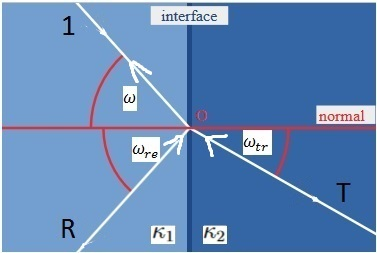
\includegraphics[height=0.85\textheight]{fres.jpg}}
\end{frame}

\begin{frame}{Френелевские условия сопряжения}
\[
\omega_{re} =\omega -2 \nu n, \quad \omega_{tr} =\psi (z,\nu) n +
\widetilde{\kappa}(z,\nu)( \omega - \nu n),   \quad \nu(z)=\omega
\cdot n(z),
\]
\[
 \widetilde{\kappa}(z,\nu) =
  \begin{cases}
 {\kappa_i}/{\kappa_j}, & \text{если} \,    \quad z \in \partial G_i \cap \partial G_j,\;   0<     \nu(z) \leq 1, \\
 {\kappa_j}/{\kappa_i}, & \text{если} \,    \quad z \in \partial G_i \cap \partial G_j,\;   -1 \leq \nu(z)  <
 0,
  \end{cases}
\]
\[
\psi(z,\nu)= \begin{cases}
 sgn(\nu) \sqrt{1- \widetilde{\kappa}^2(z,\nu) (1-\nu^2)}, & 
 \text{если} \quad 1- \widetilde{\kappa}^2(z,\nu) (1-\nu^2) \geq 0, \\
 0, \quad & \text{иначе},
  \end{cases}
\]
\[
R (z,\nu)=\frac{1}{2} (R^2_{\|}(z,\nu)+R^2_{\bot}(z,\nu)), \quad
T(z,\nu)=1-R(z,\nu),
\]
где константы $\kappa_i$ обозначают показатели преломления сред
$G_i$ и
\[
R_{\|}(z,\nu)=\frac{\widetilde{\kappa}(z,\nu)
\psi(z,\nu)-\nu}{\widetilde{\kappa}(z,\nu) \psi(z,\nu)+\nu},\quad
R_{\bot}(z,\nu)=\frac{\psi(\nu)-\widetilde{\kappa}(z,\nu)\nu}
{\psi(z,\nu)+\widetilde{\kappa}(z,\nu)\nu},
\]
\end{frame}

\begin{frame}{Интегральная форма уравнения переноса излучения}
Интегральная форма начально-краевой задачи (1)-(4) \cite{1}
\begin{equation}
I= \mathcal  E ( \mathcal S I +
J) + \mathcal P(h+ \mathcal B I^+ ).
\end{equation}
$$
{\cal S}f= 
 \int\limits_{\Omega} \sigma(r) p(r,\omega \cdot
\omega')f(r,\omega',t)d\omega',
$$
$$
\mathcal E\Phi=\int \limits^{d(r,-\omega,t)}_0 \exp
\left(- \mu_i \tau\right) \Phi(r-\tau
\omega,\omega,t-\tau/v_i)d\tau,
$$

$$
\mathcal P
\phi=\phi^-(r-d(r,-\omega,t)\omega,\omega,t-d(r,-\omega,t)/v_i)
\exp \left(-  \mu_i  d(r,-\omega,t)\right), \quad
r\in G_i,
$$

$$
h(z,\omega,t)=\left\{%
\begin{array}{ll}
    h_0(z,\omega), & \hbox{если} \; (z,\omega,t) \in X_0,  \\
    h_{ext}(z,\omega,t), & \hbox{если} \; (z,\omega,t) \in Y^-_{ext}, \\
    \end{array}%
\right.
$$
\end{frame}

\begin{frame}{Ряд Неймана}
Ряд Неймана
\[
I=\lim_{N \rightarrow \infty}I_N = \sum_{n=0}^{N}\ (\mathcal{PB} + \mathcal{ES})^n (\mathcal P h
+ \mathcal E J),
\]
рекуррентная запись
\begin{equation}
\begin{array}{c}
I_0 = \mathcal P h + \mathcal E J, \\
I_n = (\mathcal{ES} +\mathcal{PB} ) I_{n-1} + I_0,\quad n = 1, 2 \dots N.
\end{array}
\end{equation}
Интегрирование методом Монте-Карло
$$
f_n(x_n) = M[f_{n-1}(x_{n-1})] = \int k(x_n, x_{n-1})f_{n-1}(x_{n-1}), \text{где } x_{n-1} - \text{с.в.} :\rho_{x_{n-1}}(x) = k(x_n, x)
$$
\end{frame}

\begin{frame}{Генерация траектории}
Ветвящаяся траектория \cite{2,3}
\begin{multline}
{\cal I}_n(x) = \exp(-\mu_i d(r, -\omega, t)) (h(x_h) + R(x_h) {\cal I}_{n-1}^+
(x_{re}) + T(x_h) {\cal I}_{n-1}^+ (x_{tr})) +
\\ + \frac{1 - \exp(-\mu_i d(r, -\omega, t))}{\mu_i} \left(J(x_s) + \sigma_i {\cal I}_{n-1}(x_{sc})\right),
\end{multline}

\begin{equation}
{\cal I}_0(x) = \exp(-\mu_i d(r, -\omega, t)) h(x_h) +
\frac{1 - \exp(-\mu_i d(r, -\omega, t))}{\mu_i} J(x_s).
\end{equation}

Линейная траектория
\begin{equation}
{\cal I}_n(x) = \left\{
\begin{array}{ll}
   h(x_h) + {\cal I}^+_{n-1} (x_{tr}),  &\text{с вероятностью}\; p_{tr}  = T(x_h)\exp(-\mu_i  d(r,-\omega, t) ),\\
   \\
   h(x_h) + {\cal I}^+_{n-1} (x_{re}),  &\text{с вероятностью}\; p_{re} =  R(x_h)\exp(-\mu_i d(r,-\omega, t) ), \\
   \\
   \displaystyle{\frac{J(x_s)}{\mu_i}} + \displaystyle{\frac{\sigma_i}{\mu_i}} {\cal I}_{n-1} (x_{sc}), &\text{с вероятностью}\; p_{sc} = 1 - \exp(-\mu_i  d(r,-\omega, t)).
\end{array}
\right.
\end{equation}

\end{frame}

\begin{frame}{Генерация траектории}
\centering{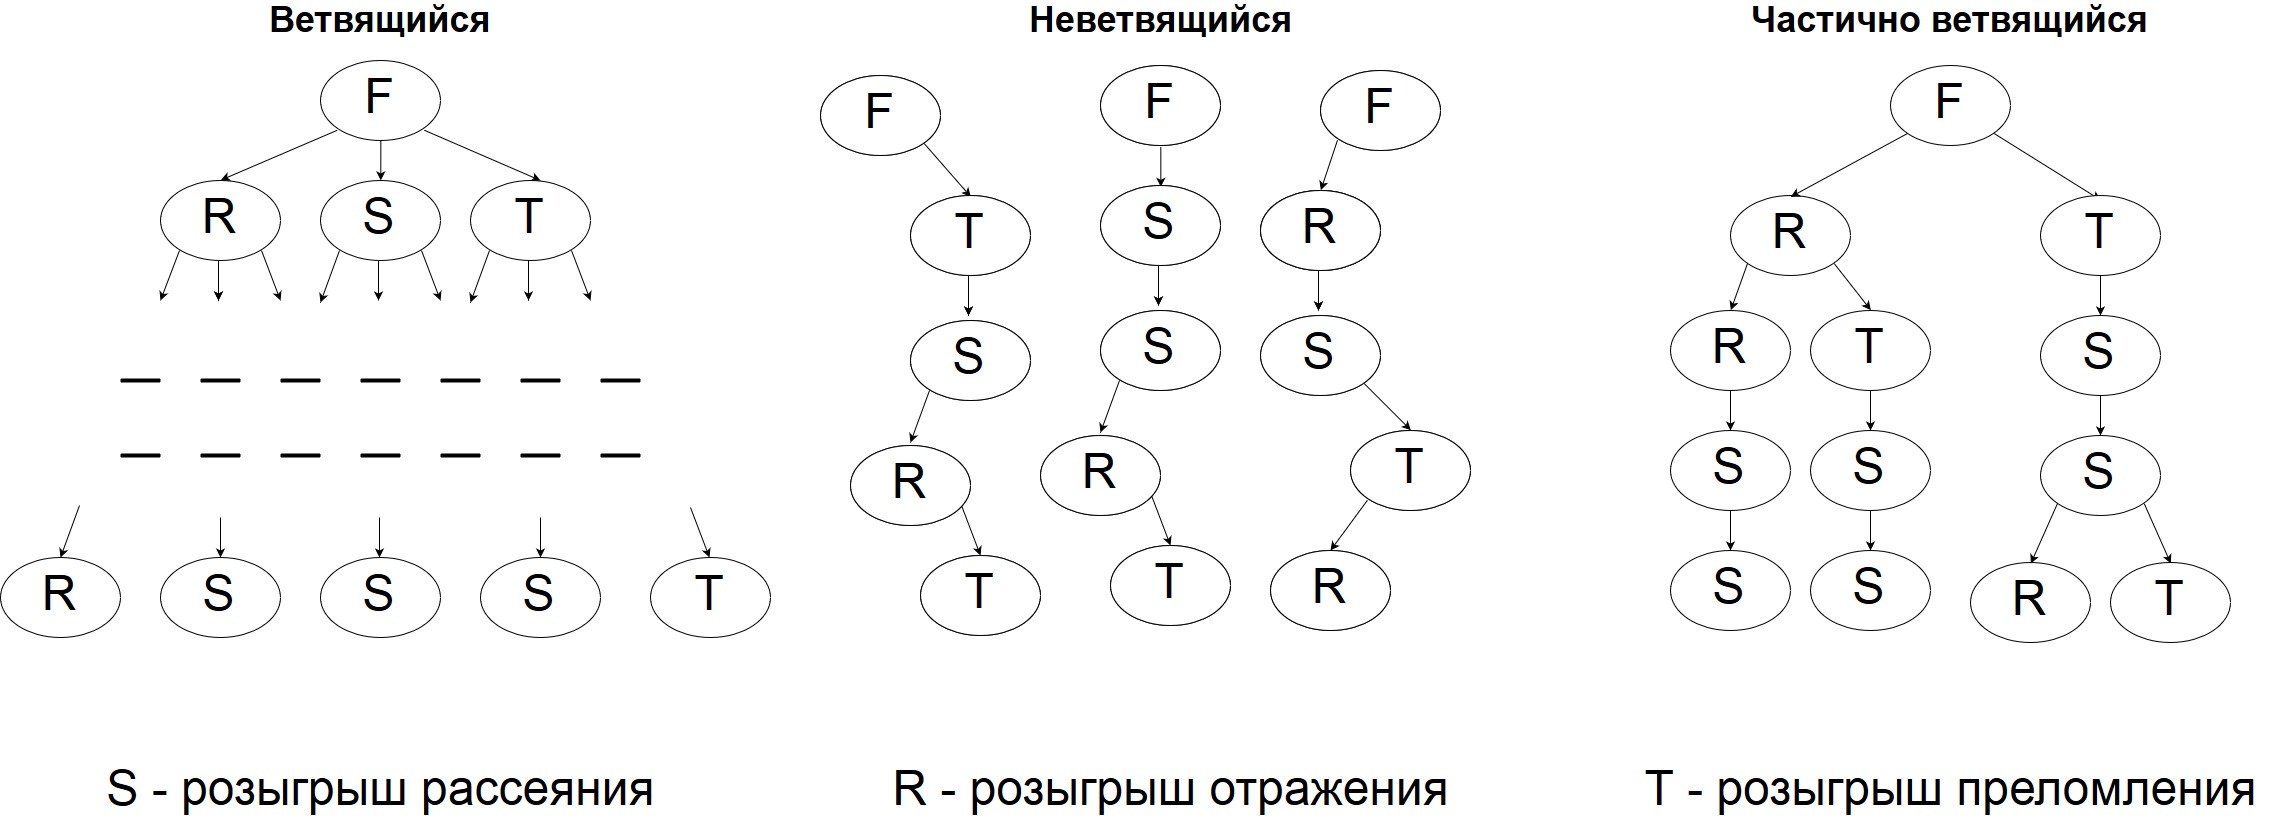
\includegraphics[width=1\textwidth]{diag1.jpg}}
\end{frame}

\begin{frame}{Тестирование}
    
\begin{table}
\begin{tabular}{c||c|c|c}
  & Тест I & Тест II & Тест III \\
\hline \hline
\begin{tabular}{l}
 \\ Подобласть 1 \\ Подобласть 2 \\ Подобласть 3 
\end{tabular}
&
\begin{tabular}{c|c|c}
$\mu$ & $\sigma$ & $\kappa$\\
\hline
 \alert{0.5}  & 0.9$\mu$ & 1\\
 \alert{0.5}  & 0.9$\mu$ & 3\\
 7.5  & 0.9$\mu$ & 10\\
\end{tabular}
&
\begin{tabular}{c|c|c}
$\mu$ & $\sigma$ & $\kappa$\\
\hline
 1.5  & 0.9$\mu$ & 1\\
 1.5  & 0.9$\mu$ & 3\\
 7.5  & 0.9$\mu$ & 10\\
\end{tabular}
&
\begin{tabular}{c|c|c}
$\mu$ & $\sigma$ & $\kappa$\\
\hline
 1.5  & 0.9$\mu$ & 1\\
 1.5  & 0.9$\mu$ & \alert{1.4}\\
 7.5  & 0.9$\mu$ & 10\\
\end{tabular}
\\
\\
\hline \hline
\begin{tabular}{l}
 \\ Ветвящийся \\ Частично \\ Неветвящийся

\end{tabular}
&
\begin{tabular}{c|c}
$S^2$ & $C$\\
\hline
0.093  & \alert{55.82}\\
 1.574  & 130.3\\
 8.463  & 212.4\\
\end{tabular}
&
\begin{tabular}{c|c}
$S^2$ &  $C$\\
\hline
0.208  & 120.6\\
 0.861 & \alert{51.76}\\
 2.380 &  60.18\\
\end{tabular}
&
\begin{tabular}{c|c}
$S^2$ & $C$\\
\hline
 0.227 & 141.6\\
 1.334 & 81.14\\
 2.510 &  \alert{65.27}\\
\end{tabular}

\end{tabular}
\end{table}
$S^2$ -- выборочная дисперсия, \\
$C$ -- трудоёмкость
\end{frame}


\begin{frame}{Сравнение CUDA реализаций частично ветвящегося и неветвящегося методов}
\centering{
  \animategraphics[controls,width=0.4\linewidth]{1}{part/b-}{1}{11}
  \animategraphics[controls,width=0.4\linewidth]{1}{non/a-}{1}{11}
}
\end{frame}


\begin{frame}{Адаптивный пороговый метод}
Введём величину ценности ветвления рассеяния в точке
$$
V_s =  W p_{sc}(p_{re}+p_{tr}),
$$
где $W$ - вес пакета дошедшего в точку
\\
ценность ветвления на границе
$$ V_b = Wp_{re}p_{tr}.  $$

Вычисляем вклад и рассеянного, и излучения с границы, если
$$ V_s > V_s^* $$
иначе разыгрываем вычисление только одного из этих слагаемых.

Если вычисляем значение излучения на границе, то проверяем условие
$$ V_b > V_b^* $$
и вычисляем оба слагаемых, если оно истинно, иначе только одно.


\end{frame}
\begin{frame}{Результаты тестирования адаптивного порогового метода}
\begin{table}
\centering
\begin{tabular}{c||c|c|c}
Алгоритм & Тест I & Тест II & Тест III \\
\hline \hline
\begin{tabular}{c}
 \\ Ветвящийся \\ Частично \\ Неветвящийся \\ Адапт. $(V^*_b=V^*_s=0.075)$
 \end{tabular}
&
\begin{tabular}{c|c}
$S^2$ & $C$\\
\hline
 0.093  & 55.82\\
 1.574  & 130.3\\
 8.463  & 212.4\\
0.521 & \alert{39.19} 
\end{tabular}
&
\begin{tabular}{c|c}
$S^2$ &  $C$\\
\hline
0.208  & 120.6\\
 0.861 & 51.76\\
 2.380 &  60.18\\
0.574 & \alert{38.38}
\end{tabular}
&
\begin{tabular}{c|c}
$S^2$ & $C$\\
\hline
 0.227 & 141.6\\
 1.334 & 81.14\\
 2.510 &  65.27\\
 0.643 & \alert{56.11} 
\end{tabular}
\end{tabular}
\end{table}
$S^2$ -- выборочная дисперсия, \\
$C$ -- трудоёмкость
\end{frame}

\begin{frame}{План работ}
  Текущая работа
  \begin{itemize}
  \item Обоснование адаптивного метода
  \item Обработка узлов в порядке уменьшения ценности \cite{4}
  \item Реализация адаптивного метода для CUDA
  \end{itemize}
  Среднесрочные планы
  \begin{itemize}
  \item Применение ветвления для интегрального слагаемого
  \item Учёт величины остаточного члена ряда Неймана для определения оптимального количества членов ряда
  \end{itemize}
  Долгосрочные планы
  \begin{itemize}
  \item Тестирование на реальных данных
  \item Практические приложения методов
  \item Исследование применимости к обратным задачам
  \end{itemize}
\end{frame}



\begin{frame}[allowframebreaks]
  \frametitle<presentation>{Библиография}
    
  \begin{thebibliography}{4}
    
  \beamertemplatebookbibitems
  % Start with overview books.

  \beamertemplatearticlebibitems
  % Followed by interesting articles. Keep the list short. 
  \bibitem{1}
    И. В. Прохоров, А. Ким.
Теоретический и численный анализ начально-краевой задачи для уравнения переноса излучения с френелевскими условиями сопряжения.
    \newblock Журнала вычислительной математики и математической физики,
    
  \bibitem{2}
    А. С. Жуплев, И. В. Прохоров, И. П. Яровенко. 
 Статистическое моделирование транспорта электронов в задачах визуализации неоднородных сред.
    \newblock Дальневост. матем. журн., 14:2 (2014), 217–230,
    2014.
  \bibitem{3}
    	Г. А. Михайлов, И. Н. Медведев.
 Оптимизация весовых методов Монте–Карло по вспомогательным переменным.
    \newblock Сиб. матем. журн., 45:2 (2004), 399–409; Siberian Math. J., 45:2 (2004), 331–340
    2004.
    
  \bibitem{4}
    D.M.O'Brien.
 Monte Carlo integration of the RTE in a scattering medium with stohastical reflecting boundary.
    \newblock J. Quant Spectrosc. Radiat. Transfer Vol. 60, No.4, pp. 573-583
    1998.
    
  \end{thebibliography}
\end{frame}

\end{document}


